% TODO translate template
\documentclass{ufsctex/ufsctex}

\usepackage{amsmath, amsfonts, amsthm, makecell, mathtools, tikz}

% English captions
\addto\captionsbrazil{
	\renewcommand{\figurename}{Figure}
	\renewcommand{\tablename}{Table}
	\renewcommand{\listfigurename}{List of Figures}
	\renewcommand{\listtablename}{List of Tables}
	\renewcommand{\contentsname}{Table of Contents}
	\renewcommand{\bibname}{REFERENCES}
}
\makeatletter
\renewcommand{\listadeabreviaturas}{
	\pretextualchapter{List of Acronyms}\@starttoc{las}}
\renewcommand{\listadesimbolos}{
	\pretextualchapter{List of Symbols}\@starttoc{lsb}}
\renewcommand{\listadealgoritmos}{
	\pretextualchapter{List of Algorithms}\@starttoc{loa}}
\makeatother

% Use standard \mathcal font
\DeclareMathAlphabet{\mathcal}{OMS}{cmsy}{m}{n}

% Create `definition' environment
\newtheorem{definition}{Definition}

% Tabular configurations
\renewcommand\theadfont{\bfseries}

% Cover info
\instituicao[a]{Universidade Federal de Santa Catarina}
\departamento[o]{Departamento de Informática e Estatística}
\curso[o]{Programa de Graduação em Ciência da Computação}
\documento[a]{Monografia}
\titulo{Reducing keys in Rainbow-like signature schemes}
\autor{Matheus Silva Pinheiro Bittencourt}
\grau{Bacharel em Ciência da Computação}
\local{Florianópolis}
\data{01}{Julho}{2019}
\orientador[Orientador]{Prof.\ Ricardo Felipe Custódio, Dr.}
\coorientador[Coorientador]{Gustavo Zambonin, Bel.}
\coordenador[Coordenador]
	{Prof.\ José Francisco Danilo de Guadalupe Correa Fletes}
\numerodemembrosnabanca{2}
\orientadornabanca{nao}
\coorientadornabanca{nao}
\bancaMembroA{
	Prof. Daniel Panario, Dr.\\
	Carleton University
}
\bancaMembroB{
	Lucas Pandolfo Perin, Me.\\
	Universidade Federal de Santa Catarina
}

\dedicatoria{Dedicatória} % TODO

\agradecimento{Agradecimentos} % TODO

\epigrafe{``\textit{Ce qui embellit le désert,
c'est qu'il cache un puits quelque part...}''}{Le Petit Prince}

\textoResumo{\textit{Inserir resumo}} % TODO
\palavrasChave{criptografia, assinatura digital, pós-quântico}

\textAbstract{\textit{Insert abstract}} % TODO
\keywords{cryptography, digital signatures, post-quantum}

\begin{document}

\pagenumbering{roman}
\capa{}
\pretextuais{}
\listadefiguras{}
\listadetabelas{}
\listadeabreviaturas{}
%\listadesimbolos{}
%\listadealgoritmos{}
\sumario{}

\chapter{Introduction}

Classic asymmetric cryptography is threatened as a result of the advance in
quantum algorithms development. The hardness of recovering private keys, for
instance, RSA\sigla{RSA}{Rivest-Shamir-Adleman} and ECDSA\sigla{ECDSA}{Elliptic
Curve Digital Signature Algorithm} keys, relies, respectively, on the hardness
of the integer factorization problem and the discrete logarithm. Quantum
algorithms, that run in polynomial-time, for solving such problems already
exist~\cite{shor1999polynomial}. Using such algorithms, recovering private keys
can be done efficiently by a sufficiently powerful quantum computer. Hence, the
most used digital signature algorithms would become insecure.

In such a scenario, cryptosystems that run on classical computers and cannot be
broken by quantum computers should be used for handling digital signatures. The
area that studies such cryptosystems is called post-quantum cryptography, and
the interest in this has emerged with the development of quantum computers. The
security of these algorithms relies on problems that are not known to be
solvable in polynomial-time, therefore, they appear to be good candidates for
use in a scenario of attackers equipped with quantum computers.

There are several classes of post-quantum cryptosystems proposed in the
literature, and each of them relies on one kind of hard problem. This work aims
to study Multivariate Public-Key Cryptosystems
(MPKCs)\sigla{MPKCs}{Multivariate Public-Key Cryptosystems}. These
cryptosystems are constructed using multivariate polynomials systems. A
Polynomial system is usually composed of polynomial equations with single
variable monomials, and can be easily solved using, for instance, Gaussian
elimination. However, with the inclusion of more variables into the monomials,
it becomes a multivariate system. The problem of solving multivariate systems
is NP-Hard~\cite{garey1979npc}. Therefore, it may be interesting to build
cryptosystems based on this trait.

Several digital signature schemes were developed based on the structure of
multivariate systems. One of the first schemes presented was the Oil and
Vinegar\sigla{OV}{Oil and Vinegar} signature scheme~\cite{patarin1997ov}, which
was broken by Kipnis and Shamir in its original
specification~\cite{kipnis1998cryptanalysis}. A subsequent
work~\cite{kipnis1999unbalanced} reparametrized it, leading to a scheme called
Unbalanced Oil and Vinegar.\sigla{UOV}{Unbalanced Oil and Vinegar} The trapdoor
introduced in the original OV is used in many other schemes. In essence, they
are similar to OV but ended up optimizing the signature, and key sizes, while
maintaining security levels. These schemes are still considered secure.

MPKCs have very efficient signature generation and verification algorithms, as
well as small signatures, in some cases, smaller than classic algorithms. The
main caveat of such schemes is that they have large public and private keys.
Various efforts were made to reduce such parts of these cryptosystems, but, to
the best of our knowledge, none of them reduced both public and private keys.
This work aims to understand the OV signature scheme, its subsequent optimized
schemes and the key reduction techniques proposed in the literature. Finally, a
new framework that allows for a reduction of both the private and the public
keys in Rainbow-like schemes is proposed.

\section{Goals and scope}

\textit{General goal:} Study and describe Rainbow-like digital signature
schemes, understand the optimizations that reduce keys and signature sizes, and
their impact on the security of the classic schemes. Observe and analyze the
impact of parameter selection for such algorithms, as this plays an important
role in efficient and fast implementations of the schemes. Analyze the
state-of-the-art schemes, to understand the strategies being used to optimize
the cryptosystems.

\textit{Specific goals:} Describe the classic OV and the UOV digital signature
schemes; Describe the Rainbow signature scheme; Introduce relevant
optimizations on Rainbow, like CyclicRainbow~\cite{petzoldt2010cyclicrainbow};
Compare and analyze the performance of the aforementioned schemes in terms of
operations needed to generate and verify signatures as well as storage
requirements. Finally, propose new optimizations on top of those schemes.

\textit{Scope:} This work will not cover other classes of post-quantum
algorithms such as code-, lattice- and hash-based cryptosystems, nor classical
asymmetric algorithms. Quantum algorithms will also not be discussed.

\section{Methodology}

% TODO improve this section
The work will be developed using the infrastructure and resources provided by
the Computer Security Laboratory (LabSEC/UFSC). A literature review will be
made to determine what is state-of-the-art in MPKCs. Recently proposed schemes
will be studied, as well as broken ones for a better understanding of the
constructions used that optimize the classic multivariate schemes. The
performance of all the schemes studied should be observed along with the impact
of the optimizations.

\chapter{Cryptographic primitives}

\textit{This chapter will be written next semester.}

\chapter{Multivariate cryptography}

In this chapter, basic foundations are given for the comprehension of the
techniques proposed in the current work. Section \ref{sec:mqsystems} contains a
description of the basic mathematical structure used to built MPKCs. Section
\ref{sec:bipolar} presents the construction used in the schemes discussed in
this work. Section \ref{sec:problems} depicts the underlying problems in which
MPKCs rely their security on. Section \ref{sec:mqschemes} describes the schemes
addressed in this study. Section \ref{sec:rainbowvariants} illustrates some
variants of the Rainbow digital signature scheme present in the literature.

\section{Systems of multivariate equations}\label{sec:mqsystems}

Standard polynomials are simply a sum of monomials, each monomial consists of a
variable and a constant that multiplies it. You may represent polynomials using
a vector that stores those constants. With multivariate polynomials, each
monomial consists of a multiplication of more than one variable and, again, a
constant. This inclusion of multiple variables to the monomials is what makes
them interesting to use in cryptosystems, since solving a system of such
polynomials is computationally hard. For the purpose of multivariate
cryptography, multivariate quadratic equations are sufficient, hence most
commonly used.

\begin{definition}
A multivariate quadratic polynomial is defined as:
\begin{equation}
p(x_1,\cdots,x_n) = \sum_{i=1}^n \sum_{j=i}^n \alpha_{ij} x_i x_j +
	\sum_{i=1}^n \beta_i x_i + \gamma
\end{equation}
where all $x, \alpha, \beta, \gamma \in \mathbb{F}$
\end{definition}

A system of polynomials is a set of polynomials that share the same variables.
It is known that, for polynomials with $n$ variables, systems that have at
least $n$ polynomials may be solvable, and it can be checked efficiently. One
of the most common methods for solving such systems is the Gaussian
elimination. Note that, not all systems with $n$ polynomials are solvable.

Systems of multivariate polynomials can be constructed as well. Opposed to the
systems explained above, solving multivariate systems is a NP-Hard
problem~\cite{garey1979npc}, even for the simplest case of quadratic
polynomials, therefore they are interesting to be used in building
cryptosystems. Specially, systems of multivariate quadratic polynomials will be
used, as the addition of more variables to the monomials does not increase the
hardness of the problem.

These systems can be seen as maps, for instance, a system $\mathcal{P}$, with
$n$ variables and $m$ equations, defines a map $\mathcal{P}:\mathbb{F}^n \to
\mathbb{F}^m$. Applying this map over a vector of variables consists of
substituting these variables into the equations and take their results as the
output of the map.

\begin{definition}\label{def:mqsystem}
A system $\mathcal{P}$ of multivariate quadratic polynomials is defined as:
\begin{equation}\label{eq:mqsystem}
\begin{split}
p^{(1)}(x_1,\cdots,x_n) &= \sum_{i=1}^n \sum_{j=i}^n \alpha^{(1)}_{ij} x_i x_j
	+ \sum_{i=1}^n \beta^{(1)}_i x_i + \gamma^{(1)} \\
p^{(2)}(x_1,\cdots,x_n) &= \sum_{i=1}^n \sum_{j=i}^n \alpha^{(2)}_{ij} x_i x_j
	+ \sum_{i=1}^n \beta^{(2)}_i x_i + \gamma^{(2)} \\
&\vdotswithin{=} \\
p^{(m)}(x_1,\cdots,x_n) &= \sum_{i=1}^n \sum_{j=i}^n \alpha^{(m)}_{ij} x_i x_j
	+ \sum_{i=1}^n \beta^{(m)}_i x_i + \gamma^{(m)}
\end{split}
\end{equation}
where all $x, \alpha, \beta, \gamma \in \mathbb{F}$
\end{definition}

Each equation of the system can be represented by an upper triangular matrix of
order $n+1$, where the element on the $i$-th line and the $j$-th column
represents the constant that multiplies the monomial $x_i x_j$. The last column
is used to represent the linear and the constant term. The $k$-th polynomial of
the system is represented by a matrix of the form:

\begin{equation}\label{eq:matrixrepresentation}
A^{(k)} =
\begin{pmatrix}
\alpha^{(k)}_{11} & \alpha^{(k)}_{12} & \alpha^{(k)}_{13} & \cdots &
	\alpha^{(k)}_{1n} & \beta^{(k)}_1 \\
0 & \alpha^{(k)}_{22} & \alpha^{(k)}_{23} & \cdots &
	\alpha^{(k)}_{2n} & \beta^{(k)}_2 \\
0 & 0 & \alpha^{(k)}_{33} & \cdots &
	\alpha^{(k)}_{3n} & \beta^{(k)}_3 \\
\vdots & \vdots & \vdots & \ddots & \vdots & \vdots \\
0 & 0 & 0 & \cdots & \alpha^{(k)}_{nn} & \beta^{(k)}_n \\
0 & 0 & 0 & \cdots & 0 & \gamma^{(k)} \\
\end{pmatrix}
\end{equation}

Furthermore, $p^{(k)}$ may be written as:
\begin{equation}
p^{(k)}(x_1,\cdots,x_n) =
	(x_1,\cdots,x_n,1) \cdot A^{(k)} \cdot (x_1,\cdots,x_n,1)^T
\end{equation}

Systems of multivariate quadratic equations can be represented and stored with
ease, as shown above. It is worth recalling that the coefficients of those
equations are elements in a small finite field, thus operating with them is
computationally efficient. Although easy to manipulate, storing these matrices
is not space efficient. A notable effort resulted in various works that reduce
the public map, \textit{e.g.} \cite{petzoldt2010cyclicrainbow}, or the private
map, \textit{e.g.} \cite{yasuda2012reducing}, but none of them reduced the key
pair simultaneously.

With the keys represented as matrices, some works introduce special structures
into these matrices, in such a way that representing them requires less space.
For instance, the series of works presented by Petzoldt introduce a framework
that enables the public key to be partially selected. Such selection is done in
a way that some special structure is introduced into the matrices, hence
reducing their space requirements. Notably, CyclicRainbow uses a cyclic
structure in the matrix representation of the public key.

\section{Bipolar construction}\label{sec:bipolar}

\begin{figure}
\centering
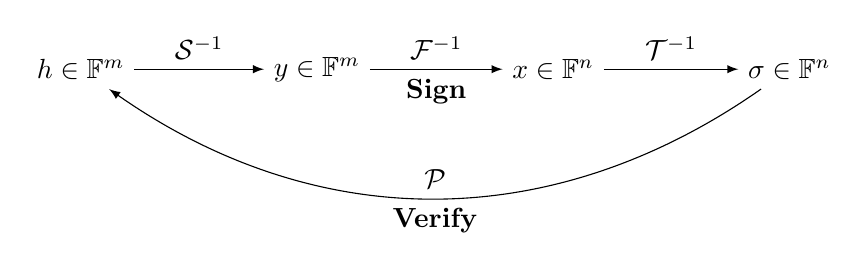
\begin{tikzpicture}
\node (h) at (0, 0) {$h \in \mathbb{F}^m$};
\node (y) at (3, 0) {$y \in \mathbb{F}^m$};
\node (x) at (6, 0) {$x \in \mathbb{F}^n$};
\node (z) at (9, 0) {$\sigma \in \mathbb{F}^n$};
\draw[-latex] (h) -- node[above]{$\mathcal{S}^{-1}$} (y);
\draw[-latex] (y) --
node[above]{$\mathcal{F}^{-1}$} node[below]{\textbf{Sign}} (x);
\draw[-latex] (x) -- node[above]{$\mathcal{T}^{-1}$} (z);
\draw[-latex] (z) to[bend left=35] node[above]{$\mathcal{P}$}
node[below]{\textbf{Verify}} (h);
\end{tikzpicture}
\caption{Flow of the bipolar construction}\label{fig:bipolar}
\end{figure}

The basic construction used in multivariate cryptosystems is based on the
composition of multiple transformations. As per Definition \ref{def:mqsystem},
a multivariate system may be used as a function
$\mathcal{F}:\mathbb{F}^n\to\mathbb{F}^m$. The central transformation of this
construction will be a system of such kind, which will contain some specific
structure such that, one can find preimages. $\mathcal{F}$ will remain secret,
and with the combination of one or more affine transformations, a public system
of equations, with no apparent structure, will be generated.

As shown in Figure \ref{fig:bipolar}, the bipolar construction consists of
three secret maps, and a public map that is derived from these three.
$\mathcal{P}$ and $\mathcal{F}$ are multivariate systems. $\mathcal{S}$ and
$\mathcal{T}$ are random invertible affine maps. In the signing procedure,
$\mathcal{F}^{-1}$ means finding one of possibly many preimages, and
$\mathcal{F}$ introduces some structure that allows one to do such. The affine
maps take care of hiding this structure by actually scrambling the variables of
the system. When generating the keys one may calculate $\mathcal{P}$ by the
composition of the secret maps $\mathcal{P} = \mathcal{S} \circ \mathcal{F}
\circ \mathcal{T}$.

Note that $n \geq m$ should hold when using the construction for digital
signature schemes. This makes the public map $\mathcal{P}$ surjective, and
ensures that for every hash $h \in \mathbb{F}^m$ there exists a signature
$\sigma \in \mathbb{F}^n$. Encryption schemes can be constructed too, in this
case $n \leq m$ should hold, thus making the map injective and ensuring that
the decryption process outputs only one plain text. Encryption schemes will not
be covered by this work.

With a hash function $\mathcal{H}:\{0,1\}^* \to \mathbb{F}^m$ one can sign a
document $d$ by calculating $h = \mathcal{H}(d)$, then, as shown in Figure
\ref{fig:bipolar}, recursively compute the signature $\sigma =
\mathcal{T}^{-1}(\mathcal{F}^{-1}(\mathcal{S}^{-1}(h)))$. This is possible due
to the fact that those maps are constructed such that they can be inverted. To
verify the signature $\sigma$ for document $d$ one can simply check if $h =
\mathcal{P}(\sigma)$ holds.

\section{Underlying computational problems}\label{sec:problems}

This section describes the problems in which multivariate cryptosystems
security rely on.

\subsection{Polynomial system solving}

Solving systems of polynomials is the basic underlying problem, since, solving
the public system is sufficient to forge new signatures.

\begin{definition}
Polynomial System Solving problem: given a system $\mathcal{P}$ as per Equation
\ref{eq:mqsystem}, find a vector $x' = (x_1',\cdots,x_n')$ such that
$p^{(1)}(x') = p^{(2)}(x') = \cdots = p^{(m)}(x') = 0$.
\end{definition}

This problem was proven to be NP-Hard~\cite[Appendix A7.2]{garey1979npc} even
for the simplest case of quadratic polynomials over $\mathbb{F}_2$. The special
case of this problem where the polynomials have degree 2 is called
\textbf{MQ-Problem}. The NP-Hardness of this problem is important due to the
fact that, it is not feasible for an attacker to solve the public map
$\mathcal{P}$ directly, hence not feasible to forge signatures this way.

\subsection{Isomorphism of polynomials}

The security of multivariate cryptosystems, due to their construction, does not
rely exclusively on the MQ-Problem. An attacker knows that the public map is
constructed by the composition of the private maps, thus one can try to
decompose the map $\mathcal{P}$ into three maps, isomorphic to the private
ones, and forge new signatures. The problem of finding such isomorphic maps is
called Extended Isomorphism of Polynomials problem.

\begin{definition}
Extended Isomorphism of Polynomials problem: given a nonlinear multivariate
system $\mathcal{P} = \mathcal{S} \circ \mathcal{F} \circ \mathcal{T}$ with
$\mathcal{F}$ belonging to some class $\mathcal{C}$ of special nonlinear
systems that can be inverted. Find $\tilde{\mathcal{S}}$, $\tilde{\mathcal{F}}$
and $\tilde{\mathcal{T}}$ such that $\mathcal{P} = \tilde{\mathcal{S}} \circ
\tilde{\mathcal{F}} \circ \tilde{\mathcal{T}}$ and $\tilde{\mathcal{F}} \in
\mathcal{C}$.
\end{definition}

With $\tilde{\mathcal{S}}$, $\tilde{\mathcal{F}}$ and $\tilde{\mathcal{T}}$ one
may forge a signature for a document $d$ by computing $\sigma =
\tilde{\mathcal{T}}^{-1}(\tilde{\mathcal{F}}^{-1}(\tilde{\mathcal{S}}^{-1}(
\mathcal{H}(d))))$ and publish it as a valid signature for the public key
$\mathcal{P}$. Recall that $\tilde{\mathcal{F}} \in \mathcal{C}$ so it can be
inverted.

Some variations of the problem with less secret maps or even ones that involve
finding the original central map $\mathcal{F}$ exist, but the extended
variation is the most generic one. In fact, solving the problem as stated
above, in polynomial time, is enough to break the Rainbow Signature
Scheme~\cite{ding2005rainbow} submitted to the NIST Post-Quantum Cryptography
Standardization Process.

Opposed to the MQ-Problem, the hardness of this problem is not well
established. Actually, on the balanced Oil and Vinegar
scheme~\cite{patarin1997ov} decomposing the public map was done efficiently by
~\cite{kipnis1998cryptanalysis}. While this problem remains an open problem,
security proofs for multivariate schemes based on the bipolar construction will
be absent. Still, MQDSS\sigla{MQDSS}{Multivariate Quadratic Digital Signature
Scheme}~\cite{chen20165} is a provably secure multivariate cryptosystem,
however it is based on a totally different construction.

\section{Multivariate digital signature schemes}\label{sec:mqschemes}

This section contains a description of the main schemes that are based on the
bipolar construction.

\subsection{Oil and Vinegar}\label{sec:ov}

The original Oil and Vinegar signature scheme was presented by
\cite{patarin1997ov}. It introduces a trapdoor that is based upon the idea of
having two sets of variables in the central map, called oil and vinegar. The
central map is constructed in such a way that the polynomials are linear in the
oil variables, that is, there are no monomials with two oil variables. With
this fact in mind, when generating a signature, one may actually linearize the
central system and solve for oil variables. A detailed description of the Oil
and Vinegar signature scheme follows.

Let $K$ be a small finite field (\textit{e.g.} $\mathbb{F}_2$). Let $o$ and $v$
be integers, such that $o$ is the number of oil variables and $v$ the number of
vinegar variables. Let $\mathcal{H}: \{0,1\}^* \to K^o$ be a cryptographic hash
function.

The private key consists of two maps $\mathcal{S}$ and $\mathcal{F}$. Let
$\mathcal{S}: K^{o+v} \to K^{o+v}$ be a random \textit{invertible} affine
transformation, it rewrites every variable as a linear combination of all other
variables. This map will be used to hide the structure of the central map. Let
$\mathcal{F}: K^{o+v} \to K^{o}$ be the central map, composed of $o$ equations
of the form:

\begin{equation}\label{eq:ovpolynomial}
y^{(k)} =
\underbrace{\sum_{i=1}^{v}\sum_{j=i}^{v} \alpha^{(k)}_{ij} x_i x_j}_{
V \times V} +
\underbrace{\sum_{i=v+1}^{v+o}\sum_{j=1}^{v} \beta^{(k)}_{ij} x_i x_j}_{
O \times V} +
\underbrace{\sum_{i=1}^{o+v} \gamma^{(k)}_{i} x_i}_{\text{linear}} +
\underbrace{\delta^{(k)}}_{\text{constant}}
\end{equation}

where $(x_1,\dots,x_v)$ are the ``vinegar'' variables and
$(x_{v+1},\dots,x_{v+o})$ are the ``oil'' variables. Note that the oil
variables are not multiplied between themselves, this will be important to find
preimages for this map when signing a message.

The public map $\mathcal{P}$ is a simple composition of the secret maps,
$\mathcal{P} = \mathcal{F} \circ \mathcal{S}$. Both $\mathcal{F}$ and
$\mathcal{P}$ are multivariate systems. $\mathcal{F}$ has the special structure
mentioned above, nevertheless $\mathcal{P}$ looks randomly built. With these
maps described, let the public/private key pair be
$(\mathcal{P},(\mathcal{S},\mathcal{F}))$.

To sign a document $d$, compute its hash value $h = \mathcal{H}(d)$, find a
preimage $(x_1,\dots,x_{o+v})$ for the map $\mathcal{F}$ such that
$(y^{(1)},\dots,y^{(o)}) = (h_1,\dots,h_o)$. Recall the structure present in
$\mathcal{F}$, setting random values to the vinegar variables makes the system
linear. Hence, finding a preimage consists of selecting vinegar variables at
random, substitute them into $\mathcal{F}$, and find the oil variables through
Gaussian elimination. If the system cannot be solved, new vinegar variables
need to be chosen. The set of variables $x$ are found such that
$\mathcal{F}(x)=h$. Next, using the map $\mathcal{S}$ the signature itself may
be computed. Recall that $\mathcal{S}$ is invertible, thus $\mathcal{S}^{-1}$
can be obtained. With both maps inverted, the signature $\sigma$ of $d$ is
published as $\sigma = \mathcal{S}^{-1}(x)$.

To verify a signature $\sigma$ of a document $d$, one can simply check if
$\mathcal{P}(\sigma) = \mathcal{H}(d)$ holds, therefore the signature is valid,
otherwise it is invalid. The equality does actually hold for valid signatures,
as $\mathcal{P}$ is a composition of the maps that were inverted in the signing
procedure. Remind that $\mathcal{P}$ is a system of multivariate equations,
hence hard to solve.

\subsection{Unbalanced Oil and Vinegar}

The original Oil and Vinegar explained in Section \ref{sec:ov} is actually
insecure due to the fact that $o = v$. It is called Balanced Oil and Vinegar
due the same amount of oil and vinegar variables. This aspect of the
cryptosystem was exploited by~\cite{kipnis1998cryptanalysis}, where a method
was introduced to efficiently forge new signatures when $o = v$. The same
authors subsequently proposed a new scheme, called Unbalanced Oil and
Vinegar~\cite{kipnis1999unbalanced}. This work proposes new parameters for the
original OV. The most common instantiation of this new scheme is the $v = 2o$
case.

\subsection{Rainbow}\label{sec:rainbow}

The Rainbow signature scheme was proposed in~\cite{ding2005rainbow}. It can be
described simply as a multilayered UOV. Actually, it is a generalization of the
UOV scheme, in other words, UOV is a single layer Rainbow instantiation. This
newly proposed scheme greatly improves space requirements in comparison to UOV.
Both public and private key sizes, as well as signatures size, are reduced for
equivalent security levels. A detailed description of the Rainbow cryptosystem
follows.

Each layer of this so called Rainbow will have its own polynomials, as well as
its own set of oil and vinegar variables. These polynomials will have the same
structure as the OV polynomials, but the layers are intrinsically connected
when constructed. Namely, $V_l$ and $O_l$ are respectively the set of vinegar
variables and the set of oil variables of the $l$-th layer. Let $u$ be the
number of layers. Let $v_1, v_2, \cdots, v_{u+1}$ be the number of vinegar
variables in each layer, such that $0 < v_1 < v_2 < \cdots < v_{u+1} = n$. Note
that the layers actually grow bigger, this is due to the fact that each set of
vinegar variables contains the vinegar variables from the previous layer, that
is $V_1 \subset V_2 \subset \cdots \subset V_{u}$. As you go deeper into the
layers, the oil variables become vinegar variables, \textit{i.e.} $V_{l+1} =
V_l \cup O_l$. Keep in mind that $|V_l| = v_l$ and $|O_l| = o_l = v_{l+1} -
v_{l}$.

The connection between variables of the layers exist in such a way that the
layers have to be inverted one after the other for the complete inversion of
the central map. To start this process, one randomly selects the first set of
vinegar variables and substitutes them, making the first layer linear. Recall
that the oil variables of some layer are part of the vinegar variables of the
subsequent layer. When the first layer is solved, the set $O_1$ can be used to
construct $V_2$ in its entirety. With known values for $V_2$ one can linearize
the second layer and solve it. Repeating this process for every layer, inverts
the whole central map. It may happen that some layer will not be solvable, in
this case, a new set $V_1$ is chosen and the inversion process starts over.
This happens with very small probability as it will be shown in section
\ref{sec:invertibility}.

Let the sets $V_l = \{x_1, \cdots, x_{v_l}\}$ be the vinegar variables of the
$l$-th layer, and $O_l = V_{l+1} - V_l$ the respective oil variables. Recall
that, each layer $l$ has $o_l = v_{l+1} - v_{l}$ equations, and thus $o_l$
equations are needed to solve for $O_l$ variables. For each layer $l$,
construct a system $\mathcal{F}_l$ composed of $o_l$ polynomials of the form:

\begin{equation}\label{eq:rainbowmap}
y^{(k)} =
\sum_{i=1}^{v_l}\sum_{j=i}^{v_l} \alpha^{(k)}_{ij} x_i x_j +
\sum_{i=v_l+1}^{v_{l+1}}\sum_{j=1}^{v_l} \beta^{(k)}_{ij} x_i x_j +
\sum_{i=1}^{v_{l+1}} \gamma^{(k)}_{i} x_i +
\delta^{(k)}
\end{equation}

for $k = v_l, \cdots, v_{l+1} - 1$ and $l = 1, \cdots, u$. Observe that the
polynomials are Oil and Vinegar polynomials, just like the ones in
Equation~\ref{eq:ovpolynomial}, and they can be solved for $O_l$ when $V_l$ has
known values. Let the central map $\mathcal{F}:K^{n} \to K^{n-v_1}$ be the
union of the $u$ layers. To hide the central map, two random invertible affine
maps will be used. Let $\mathcal{S}:K^{n-v_1} \to K^{n-v_1}$ and
$\mathcal{T}:K^{n} \to K^{n}$ be part of the private key. Publish $\mathcal{P}
= \mathcal{S} \circ \mathcal{F} \circ \mathcal{T}$ as the public key.

To sign a document $d$, using a cryptographic hash function $\mathcal{H}:
\{0,1\}^* \to K^{n-v_1}$, compute $h = \mathcal{H}(d)$. Compute $y = (y_1,
\cdots, y_{n-v_1}) = \mathcal{S}^{-1}(h)$. Solve all layers of $\mathcal{F}$ as
per the process described above, finding $x = (x_1, \cdots, x_n)$ such that
$\mathcal{F}(x) = y$. Finally, publish $\sigma = \mathcal{T}^{-1}(x)$ as the
signature for $d$.

Verifying a signature $\sigma$ for a document $d$ is as simple as checking if
$\mathcal{P}(\sigma) = \mathcal{H}(d)$ holds. Recall that, again, $\mathcal{P}$
is a multivariate system that appears to be randomly built, thus hard to solve
directly.

For illustration, Table \ref{tab:rainbowkeysizes} shows a comparison between
the key sizes of some Rainbow instances proposed in \cite[Chapter
6]{petzoldt2013thesis}. Let $m = n - v_1$ be the number of equations in Rainbow
central and public maps. The private and public key size of Rainbow-like
signature schemes is given by the formulas:

\begin{equation}
K_{pr} =
\underbrace{m^2 + m}_{\mathcal{S}} + \underbrace{n^2 + n}_{\mathcal{T}} +
\underbrace{\sum_{l=1}^{u} o_l \left(
\frac{v_l(v_l + 1)}{2} + v_l o_l + v_{l+1} + 1
\right)}_{\mathcal{F}}
\end{equation}

\begin{equation}
\begin{split}
K_{pu} &= m \left( \frac{n (n + 1)}{2} + n + 1 \right) \\
&= m \frac{(n+1)(n+2)}{2}
\end{split}
\end{equation}

These can be easily checked by looking at Equation \ref{eq:rainbowmap} and the
size of the affine maps $\mathcal{S}$ and $\mathcal{T}$. Also, the public key
size is simply the size of a multivariate system with $n$ variables and $m$
equations. The public key size formula can be checked if the matrix in Equation
\ref{eq:matrixrepresentation} is observed, as the public map is composed of $m$
matrices of such kind. OV and UOV key sizes can be calculated using $K_{pr}$
and $K_{pu}$ also, as Rainbow is a generalization of the Oil and Vinegar
schemes.

\begin{table}
\begin{center}
\begin{tabular}{|c|c|c|c|}
\hline
% header
\thead{Security level\\(bits)} & \thead{Parameters\\$(K, o_1, v_1, v_2)$}
& \thead{Public key size} & \thead{Private key size} \\ \hline
% data
80  & $(\mathbb{F}_{256}, 17, 17, 9)$   & 19208   & 25740   \\ \hline
100 & $(\mathbb{F}_{256}, 26, 22, 11)$  & 45450   & 60390   \\ \hline
128 & $(\mathbb{F}_{256}, 36, 28, 15)$  & 103704  & 139320  \\ \hline
192 & $(\mathbb{F}_{256}, 63, 46, 22)$  & 440638  & 596904  \\ \hline
256 & $(\mathbb{F}_{256}, 85, 63, 30)$  & 1086971 & 1498230 \\ \hline
\end{tabular}
\caption{Rainbow key sizes, in bytes}
\label{tab:rainbowkeysizes}
\end{center}
\end{table}

\section{Rainbow variants}\label{sec:rainbowvariants}

The cryptosystems described above have a notable space requirement. For
instance, the Rainbow public key can get up to 1.6 MB for secure
parameters~\cite[Table 2]{ding2017nist} in comparison to ECDSA's 64 bytes
public keys. This section presents some variants in the literature that reduce
Rainbow key sizes. As it will be shown, all of them reduce either the public
map or the private central map, but not both.

\subsection{Establishing a linear relation between public and private maps}
\label{sec:relation}

In~\cite{petzoldt2010cyclicrainbow} an approach is used in such way that one
can partially select the public key. It relies on an important aspect of the
schemes previously discussed. In the UOV case, it is demonstrated that the
secret map $\mathcal{S}$ actually establishes a linear relation between the
private and public coefficients of the equations. This makes it possible to
select $\mathcal{P}$ and $\mathcal{S}$ in a clever manner, such that their
representations are smaller, introducing some kind of structure like a
circulant matrix in the case of CyclicRainbow.

Recall the UOV construction of the maps $\mathcal{P} = \mathcal{F} \circ
\mathcal{S}$. To better understand this linear relation, the equations can be
simplified, without its linear and constant terms. Let $n = o + v$. Let the
$k$-th private polynomial of the system, without its linear and constant terms,
be denoted as:

\begin{equation}
y^{(k)} = \sum_{r=1}^n \sum_{s=r}^n\left(\alpha^{(k)}_{rs}x_rx_s\right)
\end{equation}

Let $\mathcal{S} \in K^{n \times n}$ be the matrix that describes the secret
affine map. The $k$-th public polynomial can be written as:

\begin{equation}\label{eq:pubpolynomial}
p^{(k)} = \sum_{r=1}^n \sum_{s=r}^n
\left[ \alpha^{k}_{rs} \sum_{i=1}^n(s_{ir}x_i) \sum_{j=1}^n(s_{js}x_j) \right]
\end{equation}

where $s_{ij}$ is the element of $\mathcal{S}$ in the $i$-th line and the
$j$-th column. The inner summations come from the matrix multiplication
operation, where the vector of $x$ variables is multiplied with $\mathcal{S}$
when the map is applied, giving a ``new'' vector of $x$ variables, that are
actually just linear combinations of the old ones. Let the public polynomial be
denoted similarly to the private one:

\begin{equation}
p^{(k)} = \sum_{r=1}^n \sum_{s=r}^n \left( \rho^{(k)}_{rs}x_rx_s \right)
\end{equation}

To establish a relation between $\alpha_{rs}$ and $\rho_{rs}$
observe the structure of equation \ref{eq:pubpolynomial} where $\alpha_{rs}$ is
multiplying two polynomials. Expanding the inner summations:

\begin{equation}
(s_{1r}x_1 + s_{2r}x_2 + \cdots + s_{nr}x_n)
(s_{1s}x_1 + s_{2s}x_2 + \cdots + s_{nr}x_n)
\end{equation}

This can be described as a new polynomial with quadratic terms, applying
distributive multiplication:

\begin{equation}\label{eq:tau}
\sum_{i=1}^{n}\sum_{j=i}^n \left( \tau^{rs}_{ij} x_i x_j \right)
\quad \mathrm{where:} \quad \tau^{rs}_{ij} =
\begin{cases}
	s_{ir} s_{is} &\mbox{if } i=j \\
	s_{ir} s_{js} + s_{jr} s_{is} &\mbox{otherwise}
\end{cases}
\end{equation}

Substituting \ref{eq:tau} into \ref{eq:pubpolynomial}:

\begin{equation}
p^{(k)} = \sum_{r=1}^n \sum_{s=r}^n
\left[
\alpha^{k}_{rs} \sum_{i=1}^{n}\sum_{j=i}^n \left( \tau^{rs}_{ij} x_i x_j \right)
\right]
\end{equation}

Therefore, a relation between private and public coefficients can be written as:

\begin{equation}\label{eq:relation}
\rho^{(k)}_{ij} = \sum_{r=1}^{n}\sum_{s=r}^n
\left( \tau^{rs}_{ij} \alpha^{k}_{rs} \right)
\end{equation}

After randomly choosing $\mathcal{S}$, equation \ref{eq:relation} depicts the
linear relation between the public ($\rho$) and private ($\alpha$)
coefficients. Hence one can choose and fix $\rho$ and find $\alpha$ using this
equation. Observe that not all public coefficients can be chosen, otherwise no
structure would be present in $\mathcal{F}$ and it could not be inverted. This
could also be used to recalculate $\mathcal{F}$ from $\mathcal{P}$ and
$\mathcal{S}$. The idea behind this relation is further expanded to Rainbow key
pairs, and is described in detail by~\cite{petzoldt2011small}. This relation
was extensively used to reduce either public or private keys, but not both.
Reducing key sizes with this strategy consists of introducing some structure
into one part of the key, such that its representation becomes smaller, and
calculating the other part using the equations above. Notable key optimizations
will be briefly discussed hereafter.

\subsection{CyclicRainbow}

CyclicRainbow~\cite{petzoldt2010cyclicrainbow} uses the relations explained in
Section~\ref{sec:relation} to structure the public key. In the key generation
step, parts of the public key matrix representation are selected such that they
form a circulant matrix.

\begin{definition}
A square circulant matrix of order $n$ is of the form:
\begin{equation}
A =
\begin{pmatrix}
a_1     & a_2    & \cdots  & a_{n-1} & a_n     \\
a_n     & a_1    & a_2     & \cdots  & a_{n-1} \\
a_{n-1} & a_n    & a_1     &         & a_{n-2} \\
\vdots  &        & \ddots  & \ddots  & \vdots  \\
a_2     & \cdots & a_{n-1} & a_n     & a_1
\end{pmatrix}
\end{equation}
\end{definition}

Such matrices allow for a compact representation. Storing the vector $(a_1,
a_2, \cdots, a_n)$ is enough to represent the matrix completely, as its
elements depict a structured repetition. Introducing this structure in parts of
the public key, when possible, reduces the representation of the public system
significantly. In fact this method allows a public key reduction factor of up
to 2.9, for secure parameters. This repetition of elements also leads up to a
repetition of operations when verifying a signature. Exploiting this common
field multiplications leads to a reduction factor of up to 2.4 in the number of
operations needed to evaluate the public map, \textit{i.e.} to verify a
signature \cite{petzoldt2013thesis}.

\subsection{RainbowLRS2}

RainbowLRS2~\cite{petzoldt2013thesis} introduces matrices generated by Linear
Recurring Sequences into the public key, just like in CyclicRainbow. To
generate an $m \times n$ matrix of this type, a vector $a = (a_1, a_2, \cdots,
a_m) \in \mathbb{F}_q^m$ of distinct elements is selected. The $i$-th row of
this matrix is:

\begin{equation}\label{eq:lrsmatrix}
A[i] = (a_i^0, a_i^1, a_i^2, \cdots, a_i^{n-1}) \qquad i = 1, \cdots, m
\end{equation}

Storing the vector $a$ is sufficient the represent the matrix $A$, since every
row can be calculated using equation \ref{eq:lrsmatrix}. Using matrices of this
fashion in the public map representation, allows for a reduction factor of up
to 3.1. Veritably, this method is pretty much similar to the one used in
CyclicRainbow, thus provides an akin improvement in space requirements. The
main difference is that CyclicRainbow uses rotations to generate each row. In
RainbowLRS2 the rows are defined by equation \ref{eq:lrsmatrix}. It is shown
in~\cite{petzoldt2013thesis} that field multiplications also repeat in the
verification process of RainbowLRS2, which allows for a speed up to a factor of
2.2.

\subsection{Circulant Rainbow}

Circulant Rainbow~\cite{peng2017circulant} introduces circulant matrices in the
central private map, in contrast to CyclicRainbow that does it on the public
map. These circulant relations will be present in very specific parts of the
central polynomials, precisely in the terms that have oil variables. Throughout
the signature generation, after inserting values into the vinegar variables,
one will have to solve a linear system as shown in section \ref{sec:rainbow}.
Due the structure introduced in the coefficients of the central map, this
system will be represented by a circulant matrix. Solving such systems can be
done more efficiently using a method described in~\cite{peng2017circulant}.
Indeed, the private key needs less space to be represented. Circulant Rainbow
has a private key 1.8 times smaller than the original Rainbow, and the
signature generation can be 2.9 times faster if the optimized method for
solving the special linear systems is used instead of the Gaussian elimination.
Notably, \cite{hashimoto2018security} discourages the use of Circulant Rainbow.
It is shown that the Kipnis-Shamir's attack~\cite{kipnis1998cryptanalysis} can
be used to recover equivalent Circulant Rainbow private keys in polynomial
time.

\subsection{NC-Rainbow}

NC-Rainbow~\cite{yasuda2012reducing} proposes the use of non-commutative rings
instead of a finite field in the central map. Further, the use of isomorphisms
between the rings and the fields need to be used in the composition of the
public map. Through this isomorphism it can be shown that a NC-Rainbow central
map is equivalent to the original Rainbow central map. In fact, it is stated
that an element $\alpha$ of a non-commutative ring $R$ can be represented by
$r$ elements in the finite field $K$. This smaller representation of the
elements in $R$ is what leads to a more compact representation of the central
map. Indeed, it is shown that the use of this technique can reduce the private
key by a factor of 4 and sign documents with 1.6 times less field
multiplications with the proposed parameters for the new scheme.

In~\cite{thomae2012quo}, it is shown that NC-Rainbow is just a special case of
introducing structures into the private central map. Additionally, it is
demonstrated that, the reduction of NC-Rainbow to the original Rainbow is not
enough to prove security. The reduction in the opposite direction is needed and
is absent in the original work. The existent reduction just provides an upper
bound for the security of the new scheme. Actually, known attacks on Rainbow
were sensibly improved for the NC-Rainbow case. The optimizations reduce the
MinRank attack complexity from $2^{288}$ to $2^{192}$ and for the HighRank, the
reduction is from $2^{128}$ to $2^{96}$. Hence, the usage of non-commutative
rings in the central map is not recommended, as it greatly decreases the
security of the original Rainbow.

% TODO equivalent keys

\chapter{Reducing private keys by reusing vinegar variables}

In chapter \ref{sec:rainbowvariants} it is shown some examples of Rainbow
variants that introduce structure in either the public key or the central map
$\mathcal{F}$. As stated above, none of these strategies could be used
simultaneously to achieve smaller key pairs. In this section, a novel
modification to the original Rainbow scheme is presented. Such modification can
reduce up to 84\% of the private key. Additionally, this optimization can be
used along with variants that introduce structure into the public key, reducing
the whole key pair by up to 71\%~\cite{zambonin2019handling}.

\section{Proposal}

It can be noted that introducing structure into the central map is generally
not well succeeded. Such schemes generally offer some vulnerability due to the
special structure in $\mathcal{F}$. With this in mind, a new general framework
to reduce private keys in Rainbow-like signature schemes is proposed. The
modification, namely Rainbow-$\eta$, consists in modifying the key generation
and the signature generation step, rather than introducing structures in the
central system of equations. Recall that the first set of vinegar variables is
chosen at random for every new signature. If this set of vinegar variables
could be reused across multiple signatures, a reduced version of the central
map, with the first set of vinegar variables substituted into the equations
could be stored, in contrast to the whole map with all variables.

Generating new keys now includes an additional step. After building
$\mathcal{F}$, the set $V_1$ is chosen randomly and then substituted into the
equations. Notice that the first layer polynomials are now linearized. $V_1$
can be substituted in the subsequent layers too. These layers remain quadratic
but with far less monomials, because the monomials that contain variables from
$V_1$ will be simplified. We store this ``linearized'' central map
$\mathcal{F'}$ along with the chosen $V_1$ for use in the signature generation
step. The rest of the key generation step remains the same. $\mathcal{P}$ is
calculated using the whole $\mathcal{F}$, but only $\mathcal{F'}$ needs to be
stored. The private key is now the tuple $(\mathcal{S}, \mathcal{F'},
\mathcal{T}, V_1)$.

To further generate new signatures, the first step of the signing procedure,
that is, chose and substitute $V_1$ into $\mathcal{F}$, is not needed anymore,
as this was done in the key generation step. The layers are inverted as
described in section \ref{sec:rainbow}. After the preimage of $\mathcal{F}$ is
found, the set $V_1$, selected in the key generation step, is used along with
the rest of the variables to compute the signature. It may happen that some
layer cannot be solvable for a given signature. Originally, when this happens,
a new set $V_1$ is chosen and the inversion process is repeated. In
Rainbow-$\eta$ this cannot be done, due to the fact that the central map
$\mathcal{F'}$ is already simplified with the previously chosen $V_1$, and
$\mathcal{F}$ is not available. With this issue in mind, henceforth three
alternatives are proposed to viabilize Rainbow-$\eta$.

\subsection{Rainbow-$\eta_1$}

In order to further regenerate the central map $\mathcal{F}$, a
PRNG\sigla{PRNG}{Pseudorandom Number Generator} seeded by $S$ can be used to
generate $\mathcal{F}$ in the key generation step. Storing $S$ with the rest of
the private key, enables the signer to regenerate $\mathcal{F}$ in the case of
the some layer not being solvable for some signature. Therefore, in the
signature procedure, if some layer fails to be solved, $\mathcal{F}$ is
regenerated completely and a new set $\tilde{V_1}$ is chosen until the first
layer becomes solvable. After $\tilde{V_1}$ is substituted into $\mathcal{F}$,
only this new simplified version of $\mathcal{F}$ needs to be kept for
subsequent signatures.

This alternative is efficient and adds only the cost of regenerating
$\mathcal{F}$ every time that some layer is not solvable, which occurs with
small probability, as it is shown in section \ref{sec:invertibility}. Also, the
cost of storing $S$ along with the private key is added.

\subsection{Rainbow-$\eta_2$}

It is show in section \ref{sec:relation} that a linear relation between the
public and private maps exist. This relation can be used to generate
$\mathcal{F}$ from $\mathcal{P}$, $\mathcal{S}$ and $\mathcal{T}$. Therefore,
in the case of the signer being unable to find a preimage for the central map,
$\mathcal{F}$ is regenerated and the signing procedure occurs just like in
Rainbow-$\eta_1$. With this method, no additional data is needed in the private
key, anyway, regenerating the central map by this manner is less efficient than
through the PRNG solution.

\subsection{Rainbow-$\eta_3$}

If the central map layers could be solved for different values, there would be
no need for new vinegar variables to be plugged in $\mathcal{F}$. This could be
achieved using a random nonce in the generation of $h$. When generating a new
signature, a random salt $r$ is chosen and $h$ is given by $h =
\mathcal{H}(\mathcal{H}(d) \| r)$. Note that now, changing $r$ changes $h$
completely.  Recall that the image $y$ is calculated by $y =
\mathcal{S}^{-1}(h)$, hence changing $r$ totally alters $y$. With this modified
hashing procedure, in the case of an unsolvable layer, $r$ is changed and the
hashing repeated, getting new values for $y$. This is done until all layers are
solvable and the signature step can follow up. The verification process is done
by checking if $\mathcal{P}(\sigma) = \mathcal{H}(\mathcal{H}(d) \| r)$ holds,
also $r$ is now part of the signature.

Actually, this method is used in the Rainbow proposal to NIST's standardization
process~\cite{ding2017nist}. This technique is used to achieve
EUF-CMA\sigla{EUF-CMA}{Existential Unforgeability under Chosen Message Attack}
security and to avoid the need of choosing new vinegar variables in the case of
some layer being unsolvable. Rainbow-$\eta_3$ is clearly more efficient than
the other variants, as it avoids the regeneration of $\mathcal{F}$. Since this
method is more efficient, and it is already used in Rainbow implementations,
the use of Rainbow-$\eta_3$ is recommended.

\section{Invertibility of the central map}\label{sec:invertibility}

As describe in section \ref{sec:rainbow}, to sign a document, $\mathcal{F}$
needs to be inverted\footnote{Note that $\mathcal{F}$ is surjective, hence
there is no inverse of this map. This inversion is actually a
``pseudo-inversion'' and it consists in finding a preimage for $\mathcal{F}$.}.
To invert $\mathcal{F}$, all layers need to be inverted individually. Inverting
each layer, after the values for the vinegar variables are substituted,
consists in solving systems of linear equations. These systems may be solvable
or not. In the case of some of these systems not being solvable, the inversion
of the central map needs to be restarted. Specially, in Rainbow-$\eta$
restarting this process adds some cost to the signature generation. In this
section, it is shown that this happens with small probability, hence the
average cost introduced by the $\eta$ variants is small.

A linear system of equations can be represented by a matrix of its
coefficients. Each line of this matrix will represent one equation. For
instance, the following system with $n$ equation and $n$ variables:

\begin{equation}
\begin{split}
y^{(1)} &= \alpha^{(1)}_1 x_1 + \alpha^{(1)}_2 x_2 + \cdots +
	\alpha^{(1)}_n x_n + \beta^{(1)} \\
y^{(2)} &= \alpha^{(2)}_1 x_1 + \alpha^{(2)}_2 x_2 + \cdots +
	\alpha^{(2)}_n x_n + \beta^{(2)} \\
&\vdotswithin{=} \\
y^{(n)} &= \alpha^{(n)}_1 x_1 + \alpha^{(n)}_2 x_2 + \cdots +
	\alpha^{(n)}_n x_n + \beta^{(k)} \\
\end{split}
\end{equation}

with all $x, y, \alpha \in \mathbb{F}_q$, can be rewritten as:

\begin{equation}\label{eq:linear}
y =
\begin{pmatrix}
\alpha^{(1)}_1 & \alpha^{(1)}_2 & \cdots & \alpha^{(1)}_n \\
\alpha^{(2)}_1 & \alpha^{(2)}_2 & \cdots & \alpha^{(2)}_n \\
\vdots & \vdots & \ddots & \vdots \\
\alpha^{(k)}_1 & \alpha^{(k)}_2 & \cdots & \alpha^{(k)}_n \\
\end{pmatrix}
\cdot x +
\begin{pmatrix}
\beta^{(1)}_n \\
\beta^{(2)}_n \\
\vdots \\
\beta^{(k)}_n \\
\end{pmatrix}
\end{equation}

with $x$ and $y$ being the column of $x$ and $y$ variables. Let $A$ be the
coefficient matrix of equation \ref{eq:linear} and $B$ the column of constant
terms, we can solve the system for a given vector $y$ by calculating:

\begin{equation}
x = A^{-1} \cdot (y - B)
\end{equation}

Actually, the system will be solvable if and only if $A$ is invertible.
Therefore, observing the probability of a randomly built matrix being
invertible shows the probability of random linear systems being
solvable\footnote{From now on, it is assumed that the linear systems generated
in the signature step, are randomly built.}.

\begin{definition}
Let $I_n$ be the identity matrix of size $n$. A matrix $A \in \mathbb{F}^{n
\times n}_q$ is invertible if and only if there exists another matrix $B \in
\mathbb{F}^{n \times n}_q$ such that $AB = BA = I_n$. $A^{-1} = B$ denotes the
inverse of $A$.
\end{definition}

It can be shown that all lines of an invertible matrix are linearly
independent. Let $A$ be an invertible matrix. For contradiction, assume that
some line of $A$ is linearly dependent of other(s). So, there exists a nonzero
column vector $x$ such that $Ax = 0$. If $A$ is invertible, then $A^{-1}Ax = 0$
can be calculated and this equality does not hold, as $x$ is nonzero.

With this fact in mind, invertible matrices can be constructed line by line,
choosing a vector that is not linearly dependent of the previously selected
ones. On the first line $l_1$ there will be a total of $q^n - 1$ choices, as
the zero vector cannot be chosen. The second line must satisfy the condition
$l_2 \neq c l_1$, since $q$ values for $c$ can be selected, the second line has
$q^n - q$ possibilities. Extending, the $k$-th line must satisfy $l_k \ne
c_1l_1 + c_2l_2 + \cdots + c_{k-1}l_{k-1}$. As there are $q^{k-1}$
possibilities for $c$ constants, the $k$-th line has $q^n - q^{k-1}$
possibilities. Multiplying all these possibilities, the probability of a random
matrix with elements in $\mathbb{F}_q$ being invertible is:

\begin{equation}
\begin{split}
p(n, q) &= \prod_{k=1}^{n} \frac{q^n - q^{k-1}}{q^n} \\
&= \prod_{k=1}^{n} \left( 1 - q^{-k} \right) \\
\end{split}
\end{equation}

Also, the probability of all layers being invertible for a given Rainbow
instance with parameters $(v_1, o_1, o_2, \ldots, o_u)$ is:

\begin{equation}
\tilde{p}(q, o_1, \ldots, o_u) =
	\prod_{l=1}^{u} \prod_{k=1}^{o_l} \left( 1 - q^{-k} \right) \\
\end{equation}

It can be observed that smaller matrices with bigger fields are more probable
to be invertible. For instance, with the parameters proposed in~\cite[Chapter
6]{petzoldt2013thesis}, using the finite field $\mathbb{F}_{16}$ and a Rainbow
instance that achieves 256-bit security level, the probability of all layers
being invertible is $\tilde{p}(16, 69, 59) \approx 87.15\%$. But using another
proposed instance, with $\mathbb{F}_{256}$ and for the same security level,
$\tilde{p}(256, 63, 30) \approx 99.21\%$. So, only in 0.79\% of the cases some
layer will not be solvable. In Rainbow-$\eta$, this probability is even
smaller, as the first layer is fixed throughout multiple signatures and it only
has a chance of not being invertible when a new set $V_1$ is chosen. Specially,
in Rainbow-$\eta_3$, as no new set $V_1$ is chosen, only the probability of the
subsequent layers need to be taken into account. It can be noted that the third
proposed variant does not add any cost to the implementation submitted
in~\cite{ding2017nist}.

\section{Similarity of multiple signatures}

Rainbow-$\eta$ fixes part of the preimage of $\mathcal{F}$, which may raise a
concern. Do multiple signatures, with the same vinegar variables, leak
information about these variables? An attacker with access to multiple
signatures that use the same set $V_1$, could derive some information about
that set if some pattern is observed across the signatures.

% TODO argument

\section{Improvement on Rainbow instances}

% TODO comparison tables
% application to existent variants

% TODO talk about proof-of-concept implementation

\chapter{Conclusion}

\textit{This chapter will be written next semester.}

% TODO article in appendix

\bibliographystyle{abnt-alf}
\bibliography{ref} % TODO fix titles, use uppercase letters

\end{document}
